\documentclass[aspectratio=169,11pt]{beamer}
\usetheme{Madrid}
\usecolortheme{default}
\usepackage{amsmath,amssymb,tikz}
\usetikzlibrary{arrows.meta,positioning,calc,fit,shapes.geometric}
\usepackage{graphicx}
\usepackage{booktabs}

\title{Why the one-branch collapse needs hypothesis $(H)$}
\subtitle{and why shotgun shelling fails\\[0.4em]
{\normalsize Graduate student seminar --- Paper A}}
\author{Alan J.\ Coppola}
\date{TopoSpine / Coppola--Weiss cyclic core}

\newcommand{\Cin}{C_{\mathrm{in}}}
\newcommand{\Cout}{C_{\mathrm{out}}}
\newcommand{\Cexp}{C_{\mathrm{exp}}}
\newcommand{\CC}{\mathrm{CC}}

\begin{document}

%-------------------------------------------------------------------
\begin{frame}
\titlepage
\end{frame}

%-------------------------------------------------------------------
\begin{frame}{One claim for the hour}
\begin{block}{What people want to believe}
A free face lets you replace the classical two-way branch
``$p$ in / $p$ out'' by a \emph{single} recursive call, and still return a
minimum-cost cover.
\end{block}
\vspace{0.6em}
\begin{alertblock}{What is actually true}
That one-branch procedure is optimal \emph{if and only if} a transport
inequality $(H)$ holds.  Cover-admissibility (what the code checks) does
\textbf{not} imply $(H)$.  Simultaneous (``shotgun'') collapse is worse still.
\end{alertblock}
\vspace{0.4em}
{\small Numbers later: all $n\le 4$ OK; two exhaustive $n=5$ failures; shotgun $5$ vs $4$.}
\end{frame}

%-------------------------------------------------------------------
\begin{frame}{Covering table and the classical two branches}
\begin{columns}[T]
\begin{column}{0.48\textwidth}
\small
Rows $=$ ON-set (minterms).\\
Columns $=$ prime implicants.\\
Entry $1$ iff the row is a face of the column.\\[0.6em]
At a cyclic core, essentials and dominance are done.
Pick a remaining column $p$:
\begin{itemize}
\item \textbf{Include $p$:} pay its weight, delete covered rows, recurse.\\
  Optimum of that branch: $\Cin$.
\item \textbf{Exclude $p$:} delete the column, recurse.\\
  Optimum of that branch: $\Cout$.
\end{itemize}
\vspace{0.4em}
Global optimum:
\[
m \;=\; \min\bigl\{\mathrm{cost}(\Cin),\,\mathrm{cost}(\Cout)\bigr\}.
\]
\end{column}
\begin{column}{0.50\textwidth}
\centering
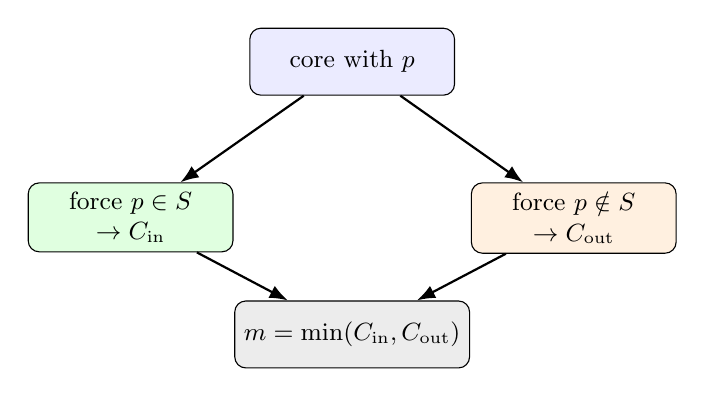
\begin{tikzpicture}[
  box/.style={draw, rounded corners, align=center, minimum width=2.6cm, minimum height=0.85cm, font=\small},
  arr/.style={-{Latex}, thick}
]
\node[box, fill=blue!8] (root) {core with $p$};
\node[box, below left=1.1cm and 0.2cm of root, fill=green!12] (in) {force $p\in S$\\$\to\Cin$};
\node[box, below right=1.1cm and 0.2cm of root, fill=orange!12] (out) {force $p\notin S$\\$\to\Cout$};
\node[box, below=2.6cm of root, fill=gray!15] (opt) {$m=\min(\Cin,\Cout)$};
\draw[arr] (root) -- (in);
\draw[arr] (root) -- (out);
\draw[arr] (in) -- (opt);
\draw[arr] (out) -- (opt);
\end{tikzpicture}
\end{column}
\end{columns}
\end{frame}

%-------------------------------------------------------------------
\begin{frame}{Free face of a collapsible cube}
\begin{columns}[T]
\begin{column}{0.55\textwidth}
A cell $p$ is \emph{collapsible} if it has a face $f<p$ of dimension
$\dim p-1$ that is not a face of any other remaining top cell.
\vspace{0.6em}

Geometry (2007 cyclic core): outer cells $1$--$6$ are collapsible;
inner $7$--$9$ are not.
\vspace{0.6em}

\begin{block}{Cover-admissible (checkable)}
Every row incident to $f$ is covered only by columns that contain $f$.
This is what \textsf{CoverAdmissibleFreeFace} tests.
\end{block}
\end{column}
\begin{column}{0.42\textwidth}
\centering
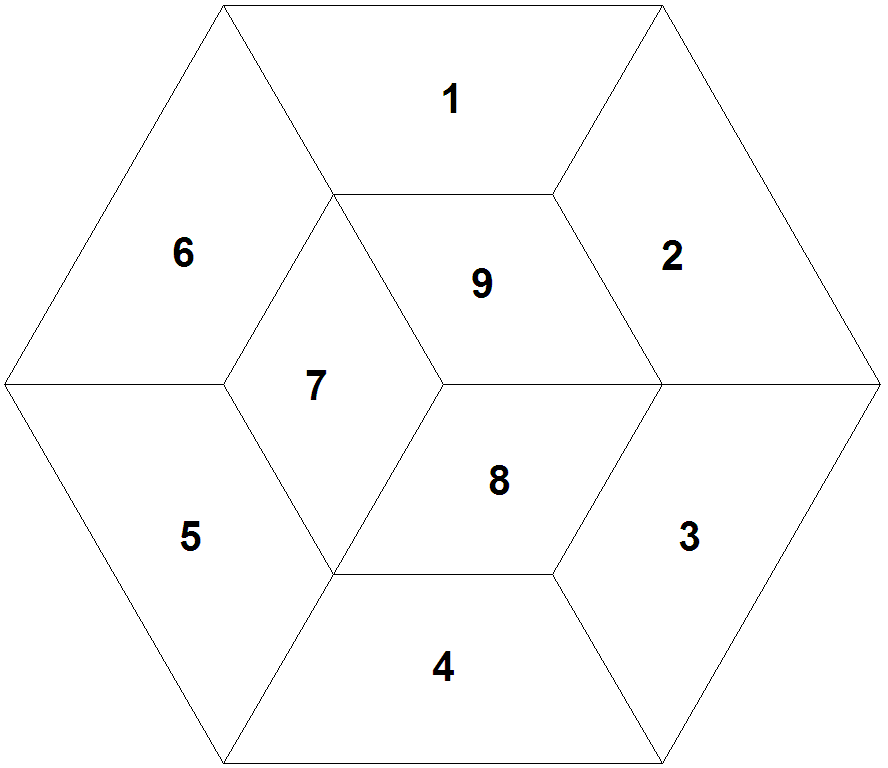
\includegraphics[width=\linewidth]{../figures/cyccore_1.png}\\[0.3em]
{\scriptsize Coppola--Weiss 2007 Fig.~1\\(geometry of that core --- not a proof of $(H)$)}
\end{column}
\end{columns}
\end{frame}

%-------------------------------------------------------------------
\begin{frame}{The quoted one-branch procedure}
\begin{block}{Collapsible Cube Reduction (as stated)}
\begin{enumerate}\setlength\itemsep{0.15em}
\item[0.] Remove $p$ from $\CC$.
\item[1.] Replace $p$ by its free faces $\mathrm{FreeFaces}(p)$ (here: one face $f$).
\item[2.] Recurse once on the expanded instance $\CC'$.
\item[3.] Let $\mathrm{CollapseCov}$ be a minimum cover of $\CC'$.
\item[4.] If $\mathrm{CollapseCov}\cap\mathrm{FreeFaces}(p)=\emptyset$: return it
  ($p$ excluded).
\item[5.] Else: return $\mathrm{Reduced}(\mathrm{CollapseCov}\cup\{p\})$
  ($p$ included; free faces dropped).
\end{enumerate}
\end{block}
\vspace{0.3em}
\centering
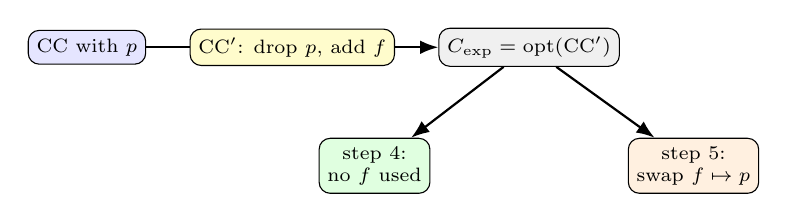
\begin{tikzpicture}[
  n/.style={draw, rounded corners, align=center, font=\scriptsize, inner sep=3pt},
  arr/.style={-{Latex}, thick}
]
\node[n, fill=blue!10] (cc) {$\CC$ with $p$};
\node[n, right=0.55cm of cc, fill=yellow!20] (exp) {$\CC'$: drop $p$, add $f$};
\node[n, right=0.55cm of exp, fill=gray!12] (sol) {$\Cexp=\mathrm{opt}(\CC')$};
\node[n, below left=0.9cm and 0.1cm of sol, fill=green!12] (ex) {step 4:\\no $f$ used};
\node[n, below right=0.9cm and 0.1cm of sol, fill=orange!12] (inc) {step 5:\\swap $f\mapsto p$};
\draw[arr] (cc) -- (exp) -- (sol);
\draw[arr] (sol) -- (ex);
\draw[arr] (sol) -- (inc);
\end{tikzpicture}
\end{frame}

%-------------------------------------------------------------------
\begin{frame}{What you get for free: expanded $\le$ exclude-$p$}
\begin{columns}[T]
\begin{column}{0.52\textwidth}
Every feasible cover of the original table that \emph{excludes} $p$ is still
feasible after the expansion (we only added a column).
\vspace{0.8em}
\[
\mathrm{cost}(\Cexp)\;\le\;\mathrm{cost}(\Cout).
\]
\vspace{0.4em}
No hypothesis needed.  Expansion never hurts the exclude-$p$ side.
\end{column}
\begin{column}{0.46\textwidth}
\centering
\begin{tikzpicture}[x=1.15cm,y=1.1cm]
\draw[-{Latex}] (0,0) -- (3.6,0) node[right] {\small cost};
\foreach \x/\lab in {1.0/{\Cexp}, 2.2/{\Cout}} {
  \draw (\x,0.12) -- (\x,-0.12);
  \node[below] at (\x,-0.15) {\scriptsize $\lab$};
}
\draw[very thick, blue!70!black] (1.0,0.35) -- (2.2,0.35);
\node[above, blue!70!black, font=\scriptsize] at (1.6,0.35) {free};
\node[above left, font=\scriptsize] at (0.1,0.9) {always};
\end{tikzpicture}
\end{column}
\end{columns}
\vspace{1em}
\begin{alertblock}{The missing comparison}
Nothing yet compares $\Cexp$ to $\Cin$ --- the best cover that \emph{includes} $p$.
That is where the argument can fail.
\end{alertblock}
\end{frame}

%-------------------------------------------------------------------
\begin{frame}{Hypothesis $(H)$: the missing inequality}
\begin{definition}[Transport hypothesis $(H)$]
\[
\mathrm{cost}(\Cexp)\;\le\;\mathrm{cost}(\Cin).
\]
\end{definition}
\vspace{0.3em}
Together with the free inequality $\mathrm{cost}(\Cexp)\le\mathrm{cost}(\Cout)$:
\[
\mathrm{cost}(\Cexp)\;\le\; m \;=\; \min\bigl\{\mathrm{cost}(\Cin),\,\mathrm{cost}(\Cout)\bigr\}.
\]
\vspace{0.6em}
\centering
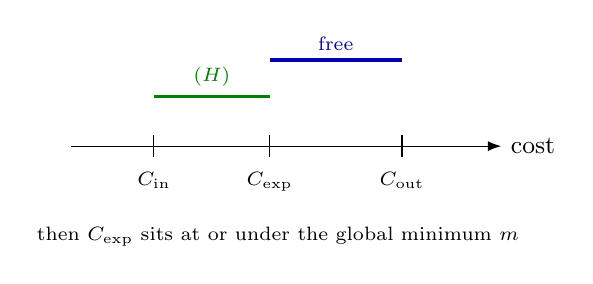
\begin{tikzpicture}[x=1.05cm,y=1.15cm]
\draw[-{Latex}] (0,0) -- (5.2,0) node[right] {\small cost};
\foreach \x/\lab in {1.0/{\Cin}, 2.4/{\Cexp}, 4.0/{\Cout}} {
  \draw (\x,0.12) -- (\x,-0.12);
  \node[below] at (\x,-0.18) {\scriptsize $\lab$};
}
% when H holds: Cin sits at or above Cexp
\draw[very thick, green!50!black] (1.0,0.55) -- (2.4,0.55);
\node[above, green!50!black, font=\scriptsize] at (1.7,0.55) {$(H)$};
\draw[very thick, blue!70!black] (2.4,0.95) -- (4.0,0.95);
\node[above, blue!70!black, font=\scriptsize] at (3.2,0.95) {free};
\node[font=\scriptsize, align=center] at (2.5,-1.0)
  {then $\Cexp$ sits at or under the global minimum $m$};
\end{tikzpicture}
\end{frame}

%-------------------------------------------------------------------
\begin{frame}{Where $(H)$ fails: $\Cin$ cheaper than the expansion}
\centering
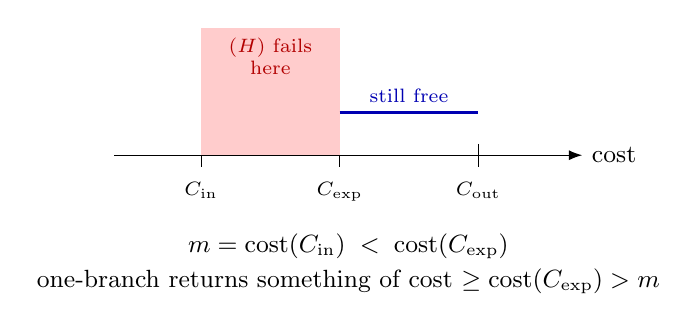
\begin{tikzpicture}[x=1.1cm,y=1.2cm]
\draw[-{Latex}] (0,0) -- (5.4,0) node[right] {\small cost};
\foreach \x/\lab in {1.0/{\Cin}, 2.6/{\Cexp}, 4.2/{\Cout}} {
  \draw (\x,0.12) -- (\x,-0.12);
  \node[below] at (\x,-0.18) {\scriptsize $\lab$};
}
\fill[red!20] (1.0,0) rectangle (2.6,1.35);
\node[red!70!black, font=\scriptsize, align=center] at (1.8,1.05)
  {$(H)$ fails\\here};
\draw[very thick, blue!70!black] (2.6,0.45) -- (4.2,0.45);
\node[above, blue!70!black, font=\scriptsize] at (3.4,0.45) {still free};
\node[font=\small, align=center] at (2.7,-1.15)
  {$m=\mathrm{cost}(\Cin)\;<\;\mathrm{cost}(\Cexp)$\\[0.2em]
   one-branch returns something of cost $\ge\mathrm{cost}(\Cexp)>m$};
\end{tikzpicture}
\vspace{0.8em}
\begin{itemize}
\item Step~4 returns an exclude-$p$ cover (cost $\ge\mathrm{cost}(\Cout)\ge\mathrm{cost}(\Cexp)>m$).
\item Step~5 returns an include-$p$ cover of cost $\approx\mathrm{cost}(\Cexp)>m$.
\end{itemize}
Neither is a global minimum.  The procedure ``works'' as code; the optimality claim is false.
\end{frame}

%-------------------------------------------------------------------
\begin{frame}{Steps 4 and 5, annotated}
\begin{columns}[T]
\begin{column}{0.48\textwidth}
\begin{block}{Step 4 --- no free face used}
$\Cexp$ uses only original columns other than $p$.\\[0.4em]
It is a feasible \emph{exclude}-$p$ cover.\\[0.4em]
If also $(H)$ held, then
$\mathrm{cost}(\Cexp)=m$, so it is optimal.\\[0.4em]
{\small Without $(H)$: only knows
$\mathrm{cost}(\Cexp)\le\mathrm{cost}(\Cout)$.}
\end{block}
\end{column}
\begin{column}{0.48\textwidth}
\begin{block}{Step 5 --- free face used}
$C'=(\Cexp\setminus\{f\})\cup\{p\}$.\\[0.4em]
Feasible because $f<p$ covers the same rows as $f$ did.\\[0.4em]
Under unit / monotone weights:
$\mathrm{cost}(C')\le\mathrm{cost}(\Cexp)$.\\[0.4em]
{\small With $(H)$: $\mathrm{cost}(C')=m$.\\
Without $(H)$: only as good as the expansion.}
\end{block}
\end{column}
\end{columns}
\vspace{0.8em}
\centering
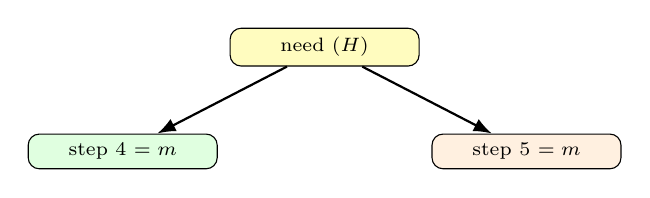
\begin{tikzpicture}[
  n/.style={draw, rounded corners, align=center, font=\scriptsize, minimum width=2.4cm},
  arr/.style={-{Latex}, thick}
]
\node[n, fill=yellow!25] (h) {need $(H)$};
\node[n, below left=0.85cm and 0.15cm of h, fill=green!12] (s4) {step 4 $=m$};
\node[n, below right=0.85cm and 0.15cm of h, fill=orange!12] (s5) {step 5 $=m$};
\draw[arr] (h) -- (s4);
\draw[arr] (h) -- (s5);
\end{tikzpicture}
\end{frame}

%-------------------------------------------------------------------
\begin{frame}{Admissibility $\neq$ $(H)$}
\begin{columns}[T]
\begin{column}{0.50\textwidth}
\begin{block}{Cover-admissible}
Local incidence check on the table.\\
Decidable.  Implemented.
\end{block}
\vspace{0.5em}
\begin{block}{Hypothesis $(H)$}
Global cost comparison after expansion.\\
Not implied by the local check.
\end{block}
\end{column}
\begin{column}{0.48\textwidth}
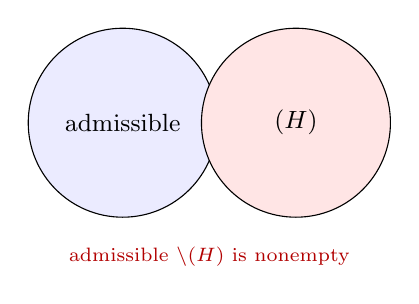
\begin{tikzpicture}[
  set/.style={draw, circle, minimum size=2.4cm, align=center, font=\small},
]
\node[set, fill=blue!8] (A) at (0,0) {admissible};
\node[set, fill=red!10] (H) at (2.2,0) {$(H)$};
\node[font=\scriptsize, red!70!black] at (1.1,-1.7)
  {admissible $\setminus(H)$ is nonempty};
\end{tikzpicture}
\end{column}
\end{columns}
\vspace{0.6em}
\begin{itemize}
\item All $n\le 4$ Boolean ON-sets: collapse-branch never disagreed with the exact optimum (fired on $330$ of the $n=4$ functions).
\item $n=5$: two exhaustive counterexamples --- costs \textbf{9 vs 8} and \textbf{8 vs 7}; admissibility held, the branch fired, $(H)$ failed.
\item Later draw of $40\,000$ functions (seed 21): $42$ disagreements with plain B\&B (rate $0.00105$).
\end{itemize}
\end{frame}

%-------------------------------------------------------------------
\begin{frame}{Can we simplify via $\mathrm{Out\_complex}$ (no free-face column)?}
\begin{block}{The 4-step $\mathrm{Out\_complex}$ procedure (unit cost $=1$)}
\begin{enumerate}\setlength\itemsep{0.15em}
\item Remove $\mathrm{FF}_c$, keeping its intersection faces inside $\mathrm{Out\_complex}$.
\item Compute $M=\mathrm{MinCov}(\mathrm{Out\_complex})$.
\item If $\mathrm{Intersection}(M,\mathrm{FF}_c)=\mathrm{FF}_c$: return $M$.
\item Else: return $\mathrm{Reduced}(M\cup\{\mathrm{FF}_c\})$.
\end{enumerate}
\end{block}
\vspace{0.4em}
\begin{columns}[T]
\begin{column}{0.48\textwidth}
\textbf{What is unconditionally true} (\textsf{OutComplex.lean}):
\begin{itemize}
\item Always returns a \emph{feasible} cover.
\item Since $R_{\mathrm{out}}\subseteq R$, $\mathrm{cost}(M)\le\mathrm{cost}(\Cout)$ is free.
\item With $\mathrm{Reduced}$, $100\%$ of $n=3$ instances ($198/198$) are exact!
\end{itemize}
\end{column}
\begin{column}{0.48\textwidth}
\textbf{Why $(H_{\mathrm{out}})$ still reappears at $n\ge 4$:}
\begin{itemize}
\item \textbf{Trap 1 (Step 4):} keeping an intersection vertex in $\mathrm{Out\_complex}$ can lock $M$ into the wrong parity (\emph{collar lock-in}).
\item \textbf{Trap 2 (Step 3):} in a cyclic core, 1D free faces have 0D shared endpoints!
\end{itemize}
\end{column}
\end{columns}
\end{frame}

%-------------------------------------------------------------------
\begin{frame}{Trap 1 --- Collar lock-in on $P_6$ (Lean \texttt{decide}-proved)}
\small
6 minterms, 5 edges in $\{0,1\}^4$.  $\mathrm{FF}_c=e_1=\texttt{-000}$ (free vertex $1000$, shared vertex $0000$):
\vspace{0.35em}
\begin{center}
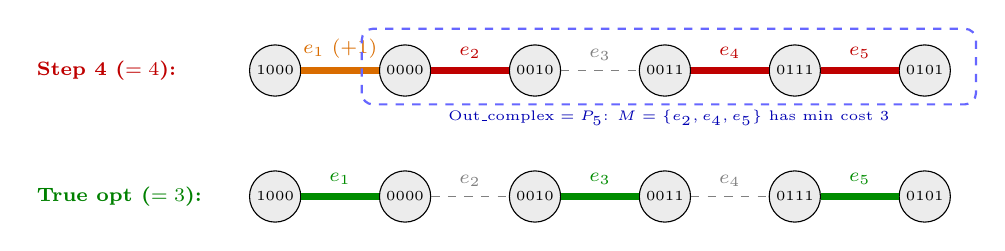
\begin{tikzpicture}[
  v/.style={circle, draw, inner sep=1.8pt, font=\tiny},
  lbl/.style={font=\scriptsize}
]
% Row 1: Out_complex + Step 4
\node[anchor=west, font=\scriptsize\bfseries, red!75!black] at (-1.5,1.25) {Step 4 ($=4$):};
\foreach \i/\b in {1/1000,2/0000,3/0010,4/0011,5/0111,6/0101} {
  \node[v, fill=gray!15] (a\i) at (\i*1.65,1.25) {$\b$};
}
\draw[line width=2.2pt, orange!85!black] (a1) -- node[above,lbl]{$e_1$ (+1)} (a2);
\draw[line width=2.2pt, red!75!black] (a2) -- node[above,lbl]{$e_2$} (a3);
\draw[dashed, gray] (a3) -- node[above,lbl]{$e_3$} (a4);
\draw[line width=2.2pt, red!75!black] (a4) -- node[above,lbl]{$e_4$} (a5);
\draw[line width=2.2pt, red!75!black] (a5) -- node[above,lbl]{$e_5$} (a6);
\draw[rounded corners, blue!60, thick, dashed] (2.75,0.82) rectangle (10.55,1.78);
\node[blue!70!black, font=\tiny] at (6.65,0.65) {$\mathrm{Out\_complex}=P_5$: $M=\{e_2,e_4,e_5\}$ has min cost $3$};

% Row 2: True min cover
\node[anchor=west, font=\scriptsize\bfseries, green!50!black] at (-1.5,-0.35) {True opt ($=3$):};
\foreach \i/\b in {1/1000,2/0000,3/0010,4/0011,5/0111,6/0101} {
  \node[v, fill=gray!15] (b\i) at (\i*1.65,-0.35) {$\b$};
}
\draw[line width=2.2pt, green!55!black] (b1) -- node[above,lbl]{$e_1$} (b2);
\draw[dashed, gray] (b2) -- node[above,lbl]{$e_2$} (b3);
\draw[line width=2.2pt, green!55!black] (b3) -- node[above,lbl]{$e_3$} (b4);
\draw[dashed, gray] (b4) -- node[above,lbl]{$e_4$} (b5);
\draw[line width=2.2pt, green!55!black] (b5) -- node[above,lbl]{$e_5$} (b6);
\end{tikzpicture}
\end{center}
\vspace{0.2em}
\begin{itemize}
\item Keeping shared vertex $0000$ in $\mathrm{Out\_complex}$ forces $e_2$, letting $M=\{e_2,e_4,e_5\}$ tie at cost $3$.
\item $\{e_1,e_2,e_4,e_5\}$ is \textbf{irredundant} ($1000\Rightarrow e_1$, $0010\Rightarrow e_2$, $0011\Rightarrow e_4$, $0101\Rightarrow e_5$): cost \textbf{4 vs 3}.
\end{itemize}
\end{frame}

%-------------------------------------------------------------------
\begin{frame}{Trap 2 --- Cyclic cores: $n\le 4$ miracle vs $n=5$ wall}
\begin{columns}[T]
\begin{column}{0.44\textwidth}
\centering
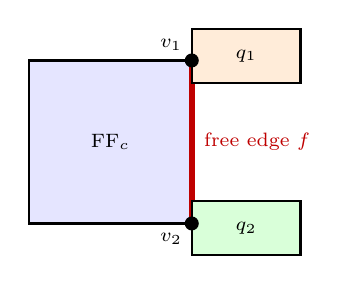
\begin{tikzpicture}[scale=1.15, every node/.style={font=\scriptsize}]
\fill[blue!10] (0,0) rectangle (1.8,1.8);
\draw[thick] (0,0) rectangle (1.8,1.8);
\node at (0.9,0.9) {$\mathrm{FF}_c$};
\draw[line width=2.3pt, red!75!black] (1.8,0) -- node[right]{free edge $f$} (1.8,1.8);
\draw[thick, fill=orange!15] (1.8,1.55) rectangle (3.0,2.15);
\node at (2.4,1.85) {$q_1$};
\draw[thick, fill=green!15] (1.8,-0.35) rectangle (3.0,0.25);
\node at (2.4,-0.05) {$q_2$};
\fill (1.8,1.8) circle (2.2pt) node[above left]{$v_1$};
\fill (1.8,0) circle (2.2pt) node[below left]{$v_2$};
\end{tikzpicture}
\vspace{0.3em}

{\scriptsize No single $q_i$ contains edge $f$,\\yet $v_1\in q_1$ and $v_2\in q_2$!}
\end{column}
\begin{column}{0.54\textwidth}
\small
After essentials are removed, \emph{every} vertex of $\mathrm{FF}_c$ is shared with some $q_i$:
\begin{itemize}
\item \textbf{Keep shared vertices ($R_{\mathrm{out}}=R$):} $M$ covers all of $R$, so Step~3 \emph{always} fires and returns $\Cout$.\\
  {\scriptsize Fails $192/1\,544$ times on $n=4$ ($9\times 9$: cost $5$ vs $4$).}
\item \textbf{Drop all $\mathrm{FF}_c$ rows ($R_{\mathrm{out}}=R\setminus\mathrm{FF}_c$):} Step~4 returns $\Cin$.
  \begin{itemize}
  \item \textbf{$n\le 4$:} $0/1\,544$ errors across all $4\,368$ collapsible columns!
  \item \textbf{$n=5$:} fails when unique opt excludes $\mathrm{FF}_c$ ($9\times 9$, $\mathrm{FF}_c=\texttt{1--00}$: $\Cin=5$ vs $\Cout=4$).
  \end{itemize}
\end{itemize}
\end{column}
\end{columns}
\end{frame}

%-------------------------------------------------------------------
\begin{frame}{Shotgun: collapse several pairs at once}
\begin{columns}[T]
\begin{column}{0.48\textwidth}
\textbf{Sequential}
\begin{enumerate}\setlength\itemsep{0.2em}
\item Collapse one admissible pair.
\item Reduce (essentials, dominance).
\item Collapse the next.
\end{enumerate}
\vspace{0.4em}
Between steps the table can force columns and delete rows.  That re-reduction is load-bearing.
\end{column}
\begin{column}{0.48\textwidth}
\textbf{Shotgun (batch)}
\begin{enumerate}\setlength\itemsep{0.2em}
\item Pick several admissible pairs at once.
\item Remove all those parents; insert all those faces.
\item Decode face $\mapsto$ parent at the end.
\end{enumerate}
\vspace{0.4em}
No intermediate reduction.  Even a coverability guard (``safe'') does not restore optimality.
\end{column}
\end{columns}
\vspace{0.7em}
\centering
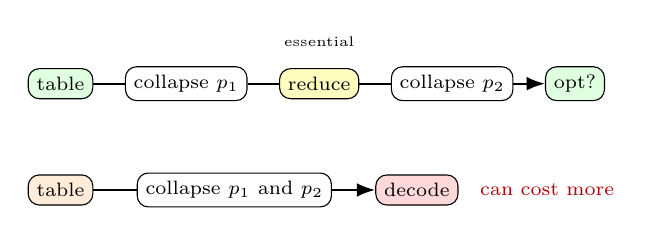
\begin{tikzpicture}[
  n/.style={draw, rounded corners, align=center, font=\scriptsize, inner sep=3pt},
  arr/.style={-{Latex}, thick}
]
\node[n, fill=green!12] (s0) {table};
\node[n, right=0.4cm of s0] (s1) {collapse $p_1$};
\node[n, right=0.4cm of s1, fill=yellow!25] (r) {reduce};
\node[n, right=0.4cm of r] (s2) {collapse $p_2$};
\node[n, right=0.4cm of s2, fill=green!12] (ok) {opt?};
\draw[arr] (s0)--(s1)--(r)--(s2)--(ok);
\node[above=0.15cm of r, font=\tiny] {essential};
\begin{scope}[yshift=-1.35cm]
\node[n, fill=orange!15] (b0) {table};
\node[n, right=0.55cm of b0] (b1) {collapse $p_1$ and $p_2$};
\node[n, right=0.55cm of b1, fill=red!15] (bad) {decode};
\draw[arr] (b0)--(b1)--(bad);
\node[right=0.15cm of bad, font=\scriptsize, red!70!black] {can cost more};
\end{scope}
\end{tikzpicture}
\end{frame}

%-------------------------------------------------------------------
\begin{frame}{Shotgun witness: optimum $4$, batch returns $5$}
\begin{itemize}
\item Smallest guarded counterexample: $7$ columns, $14$ rows (an $n=4$ ON-set).
\item Exact / plain B\&B / sequential collapse-branch: cost \textbf{4}.
\item Shotgun with the \texttt{safe} rule (row-disjoint faces + coverability guard): cost \textbf{5}, still feasible.
\end{itemize}
\vspace{0.6em}
\centering
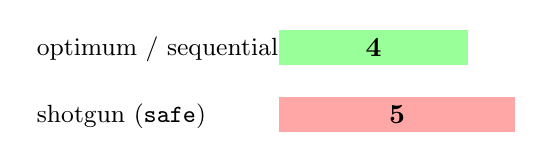
\begin{tikzpicture}[
  bar/.style={draw, minimum height=0.55cm, font=\small},
]
\node[anchor=west] at (0,1.2) {\small optimum / sequential};
\fill[green!40] (3.2,1.0) rectangle (5.6,1.45);
\node at (4.4,1.225) {\textbf{4}};
\node[anchor=west] at (0,0.35) {\small shotgun (\texttt{safe})};
\fill[red!35] (3.2,0.15) rectangle (6.2,0.6);
\node at (4.7,0.375) {\textbf{5}};
\end{tikzpicture}
\vspace{0.8em}
\begin{block}{Broader audit ($n=4$, all nontrivial batches)}
\begin{itemize}
\item Guarded (\texttt{safe}): $33/864$ cost mismatches, $0$ infeasible reduced tables.
\item Naive rules: $672/864$ mismatches \emph{and} $672$ reduced tables left with an uncovered row.
\end{itemize}
\end{block}
\end{frame}

%-------------------------------------------------------------------
\begin{frame}{What the code certifies instead}
\begin{columns}[T]
\begin{column}{0.52\textwidth}
\begin{block}{Certified covers}
Plain branch-and-bound.\\
When $\le 16$--$22$ columns remain, an exhaustive oracle re-checks the cost.
\end{block}
\vspace{0.5em}
\begin{block}{Audited comparators}
\begin{itemize}
\item Collapse-branch (records whether it agreed).
\item Shotgun (certificate rejected if it claims optimality).
\end{itemize}
\end{block}
\end{column}
\begin{column}{0.46\textwidth}
\begin{alertblock}{Open for the room}
A \emph{checkable} condition that implies $(H)$ on minterm covering tables.\\[0.5em]
Candidates tried (equal row support, vertex faces, edge parents, face covers $\le 1$ row): vacuous or still refuted.
\end{alertblock}
\end{column}
\end{columns}
\vspace{0.8em}
{\small Paper A: \emph{Certified Cyclic-Core Transformations for Minimum Covering}.\\
TopoSpine ledger C2 (disproved as implemented), C9 (shotgun disproved).}
\end{frame}

%-------------------------------------------------------------------
\begin{frame}{Take-away}
\begin{enumerate}
\item The one-branch picture --- both via free-face columns and via $\mathrm{Out\_complex}$ --- is a \textbf{reduction to $(H)$ / $(H_{\mathrm{out}})$}, not an unconditional theorem.
\item On $P_6$ ($n=4$), keeping the shared vertex in $\mathrm{Out\_complex}$ locks in cost $4$ vs $3$ (Lean \texttt{decide}-checked); on cyclic cores, forcing $\mathrm{FF}_c$ in works on $100\%$ of $n\le 4$ ($1\,544$ cores) and breaks at $n=5$ ($5$ vs $4$).
\item Shotgun skips the intermediate reduction that sequential collapse uses; even a feasibility guard leaves optimality on the floor ($5$ vs $4$).
\item The implementation is honest about all three: plain B\&B certifies; collapse, $\mathrm{Out\_complex}$, and shotgun are audited.
\end{enumerate}
\vspace{1em}
\centering
\large Questions.
\end{frame}

\end{document}
